\begin{center}
  \Large
  \textbf{BIOGRAFI PENULIS}
\end{center}

\addcontentsline{toc}{chapter}{BIOGRAFI PENULIS}

\vspace{2ex}

\begin{wrapfigure}{L}{0.3\textwidth}
  \centering
  \vspace{-3ex}
  % Ubah file gambar berikut dengan file foto dari mahasiswa
  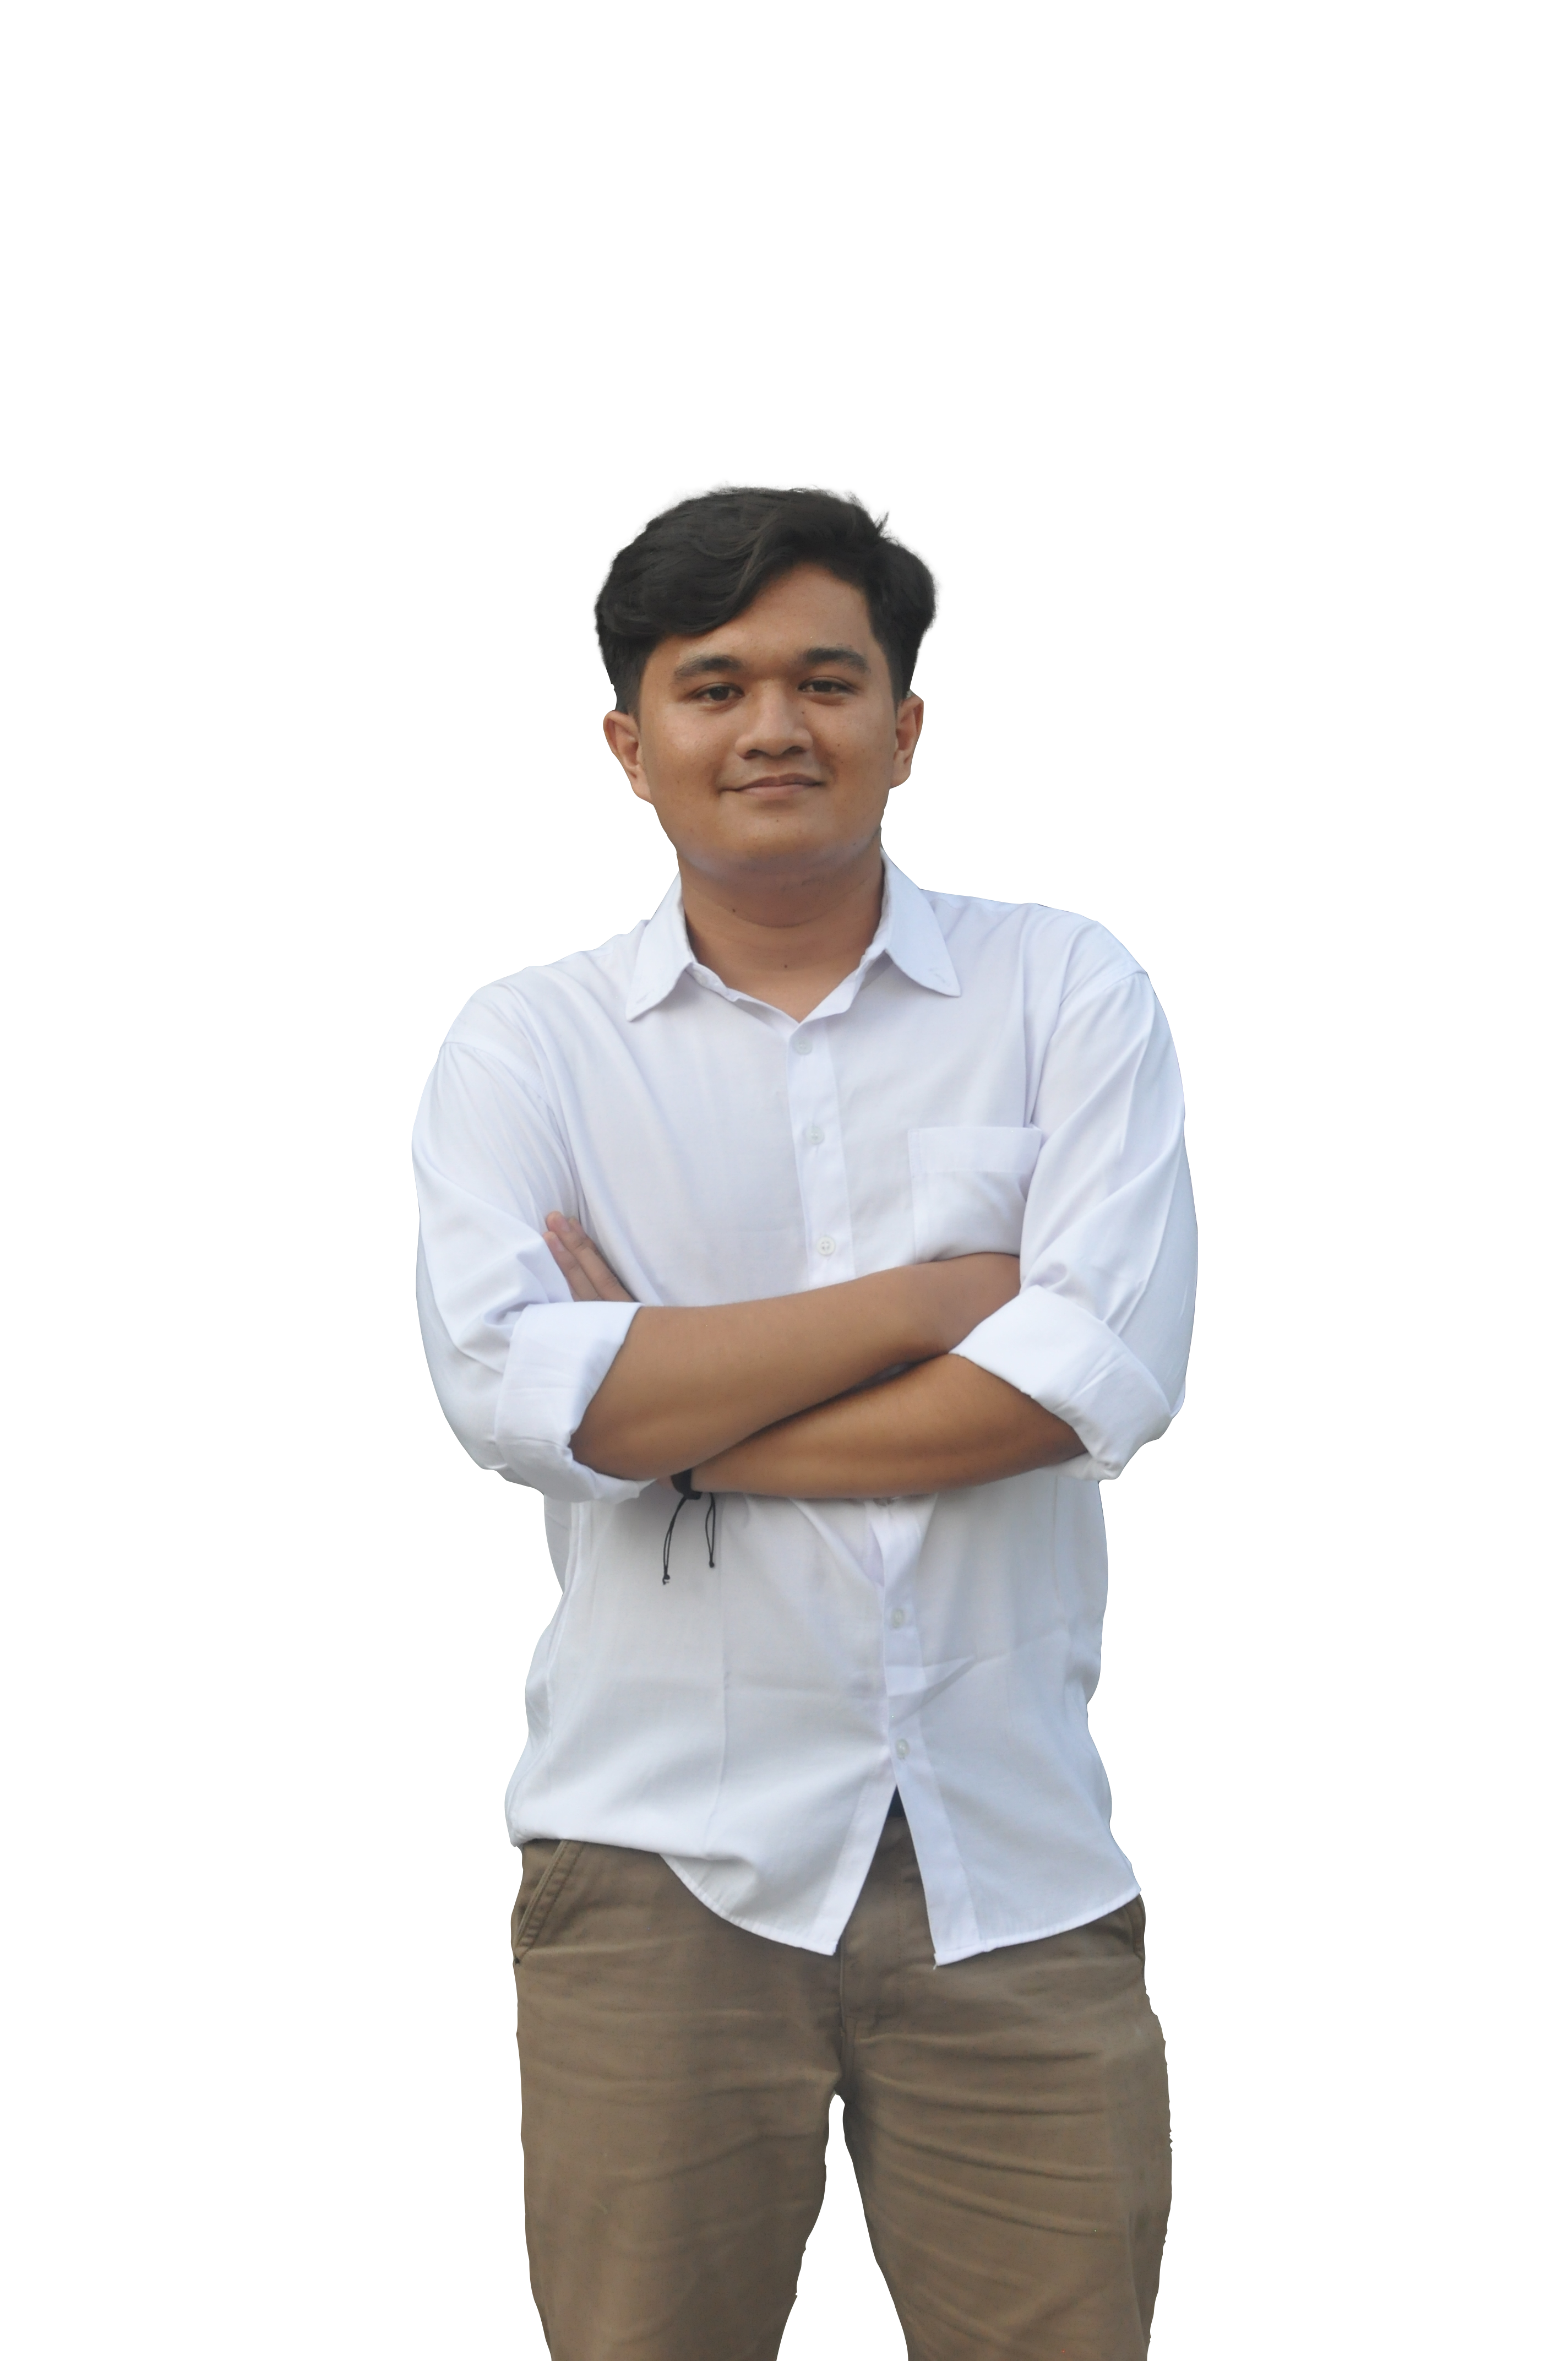
\includegraphics[width=0.3\textwidth]{gambar/joe.png}
  \vspace{-4ex}
\end{wrapfigure}

% Ubah kalimat berikut dengan biografi dari mahasiswa
\name{}, adalah penulis penelitian ini. Lahir dari Pasangan Bapak E. Napitupulu dan A. Manik dan merupakan anak ke 2 dari 3 bersaudara. Penulis lahir di Parapat tepatnya di Kabupaten Simalungun Sumatera Utara pada 08 November 2002. Penulis memulai pendidikan formal di SD Negeri N2091462 Parapat(2008-2014),SMP Negeri 1 Girsang Sipangan Bolon(2014-2017),SMA Swasta Rk. Bintang Timur Pematang Siantar(2017-2020). Kemudian setelah menyelesaikan pendidikan SMA di Pematang Siantar, Penulis melanjutkan studi S1 di Institut Teknologi Sepuluh Nopember di departemen Teknik Komputer. Penulis aktif berorganisasi di BEM Fakultas Teknologi Elektro dan Informatika Cerdas ITS(2022-2024) dan Juga merupakan anggota GenBI tahun 2022-2024. Penulis memiliki minat yang tinggi dibidang elektrikal dan dunia Internet Of Things(IoT). Pengalaman terakhirnya pada dibidang yang ditekuni yaitu internship atau magang selama 6 bulan di PT. Kalbe Farma Tbk, sebagai Industrial IoT and Automation Engineer.